% Standard Article Definition
\documentclass[]{article}

% Page Formatting
\usepackage[margin=1in]{geometry}
\setlength\parindent{0pt}

% Graphics
\usepackage{graphicx}

% Math Packages
\usepackage{physics}
\usepackage{amsmath, amsfonts, amssymb, amsthm}
\usepackage{mathtools}

% Extra Packages
% \usepackage{pdfpages}
\usepackage{hyperref}
% \usepackage{listings}

% Section Heading Settings
% \usepackage{enumitem}
% \renewcommand{\theenumi}{\alph{enumi}}
\renewcommand*{\thesection}{Problem \arabic{section}}
\renewcommand*{\thesubsection}{\alph{subsection})}
\renewcommand*{\thesubsubsection}{}%\quad \quad \roman{subsubsection})}

\newcommand{\Problem}{\subsubsection*{\textbf{PROBLEM:}}}
\newcommand{\Solution}{\subsubsection*{\textbf{SOLUTION:}}}
\newcommand{\Preliminaries}{\subsubsection*{\textbf{PRELIMINARIES:}}}

%Custom Commands
\newcommand{\N}{\mathbb{N}}
% \newcommand{\Z}{\mathbb{Z}}
% \newcommand{\Q}{\mathbb{Q}}
\newcommand{\R}{\mathbb{R}}
\newcommand{\C}{\mathbb{C}}

% \newcommand{\SigAlg}{\mathcal{S}}

% \newcommand{\Rel}{\mathcal{R}}

% \newcommand{\toI}{\xrightarrow{\textsf{\tiny I}}}
% \newcommand{\toS}{\xrightarrow{\textsf{\tiny S}}}
% \newcommand{\toB}{\xrightarrow{\textsf{\tiny B}}}

% \newcommand{\divisible}{ \ \vdots \ }
\newcommand{\st}{\ : \ }

% Theorem Definition
\newtheorem{definition}{Definition}
\newtheorem{assumption}{Assumption}
\newtheorem{theorem}{Theorem}
\newtheorem{lemma}{Lemma}
\newtheorem{proposition}{Proposition}
\newtheorem{remark}{Remark}
% \newtheorem{example}{Example}
% \newtheorem{counterExample}{Counter Example}


%opening
\title{
    MECH 6326 - Optimal Control and Dynamic Programming \\ 
    Homework 1
}
\author{Jonas Wagner\\ jonas.wagner@utdallas.edu}
\date{2023, Febuary 10\textsuperscript{st}}

\begin{document}

\maketitle

\tableofcontents

% Problem 1 ----------------------------------------------
\newpage
\section{}
\Problem
Find and research an example (ideally from your own research experience/interests, or from an actual company/startup) of a problem of multi-step decision making under uncertainty in the real world. 
Write a short narrative that briefly describes 
i) the use (or potential use) of closed-loop feedback control/recourse due to uncertain factors affecting performance and operation and 
ii) the performance objectives and operation of the system, including the system dynamics, system states, inputs, outputs, and stochastic disturbances and other uncertainties. 
Comment specifically on any stochastic uncertainties and how you might go about collecting data to describe their probability distribution. 
Explain why an open-loop controller may not be sufficient and what are the advantages of using closed-loop feedback/recourse by utilizing knowledge of the system state and/or realizations of uncertain parameters at each time instant

\Solution
Since I have many examples that could fit this description I will take one of the more complicated ones to touch base on each of the questions.

\textbf{NOVA Vehicle} \cite{mech6323FinalProject}
Specifically I have a bicycle model of the vehicle that I've been using in research.

I can copy over my entire report from Robust Control on the various uncertainties and how we model this (in continuous time, I have been working with a DT model for a lateral motion in research) but I'll instead just have the link here:
\url{https://github.com/jonaswagner2826/MECH6323/blob/master/FinalProject/Report/MECH6323_FinalProject.pdf}

The TLDR for the system is included with the \figurename \ref{fig:3dof_bike_model} and the nonlinear dynamics in \eqref{eq:full_nonlin_eq}.

\begin{figure}[b]
    \centering
    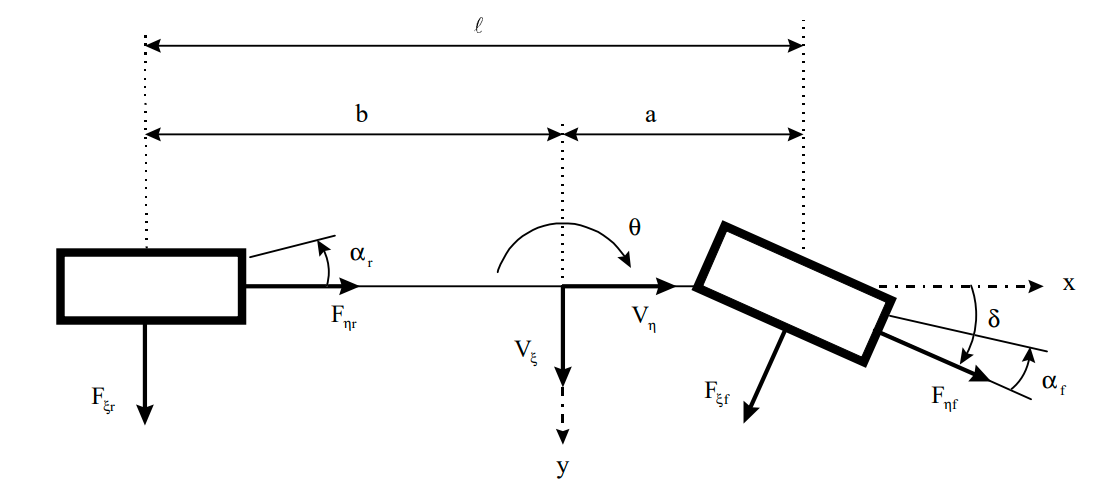
\includegraphics[width=0.5\textwidth]{figs/3dof_model_diag.png}
    \caption{3 DOF Bicycle Model}
    \label{fig:3dof_bike_model}
\end{figure}

As for the specific questions asked, here's a bit of a narrative:

\textbf{(i)}
For `simpler' vehicle motions (lane-keeping) we can split the problem into partially independent longitudinal (`Speed/Position') and lateral (`Side-to-side/steering') controllers.
Each of these can benefit from a closed-loop controller that accounts for many areas of system and sensor noises.

\textbf{(ii)}

\begin{equation}\begin{cases}
    I \ddot{\theta}     &= a F_{\eta f} \delta + b F_{\zeta f} - b F_{\zeta r}\\
    m (\dot{V_{\zeta}} + V_\eta \dot{\theta}) &= F_{\eta f} \delta + F_{\zeta f} + F_{\zeta r}\\
    m(\dot{V_{\eta}} + V_\zeta \dot{\theta}) &= F_{\eta f} + F_{\eta r} + F_{\zeta f} \delta\\
    \dot{x} &= -V_{\zeta} \sin(\theta) + V_{\eta} \cos(\theta)\\
    \dot{y} &= V_{\eta} \cos(\theta) + V_{\zeta} \sin(\theta)
\end{cases}\label{eq:full_nonlin_eq}\end{equation}
The global system coordinates are $(x, y, \theta)$, 
longitudinal $(\eta)$ and lateral $(\zeta)$ velocities $(V_\eta, V_\zeta)$,
longitudinal and lateral forces for the front and rear as $(F_{\eta f},F_{\eta r},F_{\zeta f},F_{\zeta r})$,
steering angle of $\delta$, 
and with physical parameters that are uncertain.

The following is the implementation of the nonlinear dynamics equations \eqref{eq:full_nonlin_eq} in state space with the state vector, $x = [\dot{\theta}, V_\zeta, V_\eta, x, y, \theta]^T$, and input vector $u = [\delta, F_{\eta f}, F_{\eta r}, F_{\zeta f}, F_{\zeta r}]^T$. 
\begin{equation}\begin{cases}
    \dot{x}_1 &= \frac{a F_{\eta,f} \delta + b F_{\zeta,f} - b F_{\zeta,r}}{I}\\
    \dot{x}_2 &= \frac{F_{\eta,f} \delta + F_{\zeta,f} - F_{\zeta,r}}{m} - x_3 x_1\\
    \dot{x}_3 &= \frac{F_{\eta,f} + F_{\eta,r} - F_{\zeta,r}\delta}{m} - x_2 x_1\\
    \dot{x}_4 &= -x_2 \sin(x_6) + x_3 \cos(x_6)\\
    \dot{x}_5 &= x_2 \cos(x_6) + x_3 \sin(x_6)\\
    \dot{x}_6 &= x_1
\end{cases}\end{equation}

In addition to any model uncertainty (which can be modeled as system noise) the stocastic uncertainty is generated from sensor measurments and nonlinearities of actuators. 
See the report for all the specifics on the sensors and actuators which have explinations on the uncertainty for each.

The advantages of the of a closed-loop operation (and additionally the dynamic updating of parameters) is a very long list so I'm going to neglect explaining them, but it essentially is a staight-foward answer of: uncertainty makes it act different then expected so the open-loop will likely fail.


% Problem 2 ----------------------------------------------
\newpage
\section{}
Consider the DT L(TI) stochastic dynamical system 
\begin{equation}
    x_{k+1} = A x_k + B u_k + w_k
\end{equation}
where $x_k \in \R^n$, $u_k \in \R^m$, and $w_k \sim \mathcal{N}(0,W)$ is an iid signal.
Suppose $x_0 \sim \mathcal{N}(0,X_0)$ is another iid random variable.
The control input is given by a linear feedback control policy $u_k = K x_k$, with $K \in \R^{m \cross n}$.

% 2a ---------------------------------------------------------------
\subsection{}
\Problem
Let the state mean be defined as $\mu_k := E[x_k]$ and state second moment matrix defined as $\Sigma_k := E[x_k x_k^T]$.
Derive the dynamics for the state mean and second moment matrix,
(i.e.) write $\mu_{k+1}$ and $\Sigma_{k+1}$ in terms of $\mu_k$, $\Sigma_k$ and the given problem data $(A, B, K, W, X0)$.

\Solution
Since the system is LTI, the propagation of the mean and variance can be directly computed as the expected value of the update equations.

In the closed loop we have \[x_{k+1} = (A+BK) x_k + w_k\]

\textbf{State mean update:}
\begin{align*}
    \mu_{k+1} = E[x_{k+1}] 
        &= E[(A+BK) x_k + w_k]\\
        &= E[(A+BK) x_k] + E[w_k]\\
        &= (A+BK) E[x_k] + (0)\\
        &= (A+BK) \mu_k
\end{align*}

\textbf{State covariance update:}
\begin{align*}
    \Sigma_{k+1} = E[x_{k+1} x_{k+1}^T]
        &= E[((A+BK)x_k + w_k)((A+BK)x_k + w_k)^T]\\
        &= E[((A+BK)x_k + w_k)(x_k^T(A+BK)^T + w_k^T)]\\
        &= E[(A+BK)x_k x_k^T (A+BK)^T + (A+BK)x_k w_k
            + w_k x_k^T(A+BK)^T + w_k w_k^T]\\
        &= E[(A+BK)x_k x_k^T (A+BK)^T] + E[(A+BK)x_k w_k]
            + E[w_k x_k^T(A+BK)^T] + E[w_k w_k^T]\\
        &= (A+BK)E[x_k x_k^T](A+BK)^T + (A+BK)E[x_k w_k]
            + E[w_k x_k^T](A+BK)^T + E[w_k w_k^T]
\intertext{since $x_k$ and $w_k$ are independent,}
        &= (A+BK)E[x_k x_k^T](A+BK)^T + (A+BK)E[x_k] E[w_k]
            + E[w_k] E[x_k^T](A+BK)^T + E[w_k w_k^T]\\
        &= (A+BK)(\Sigma_k)(A+BK)^T + (A+BK)(\mu_k)(0)
            + (0)(\mu_k)(A+BK)^T + (W)\\
        &= (A+BK)\Sigma_k(A+BK)^T + W
\end{align*}

% 2b ---------------------------------------
\subsection{}
\Problem
Suppose $n=m=1$.
Derive and expression for the steady state second moment $\Sigma_\infty := \lim_{k\to\infty} \Sigma_k$.
Under what conditions does this converge to a finite value?
In this case is $\lim_{k\to\infty} \mathbf{P}(x_k \geq 3 \sqrt{\Sigma_\infty})$; (i.e.) the probability that in steady state, the state takes a value greater than $3\sqrt{\Sigma_\infty}$?

\Solution
Steady state occurs when $\Sigma_{k+1} = \Sigma_k = \Sigma_\infty$.

\begin{align*}
    \Sigma_\infty &= (A+BK)\Sigma_\infty(A+BK)^T + W\\
\intertext{since $(A+BK)$ is a scaler,}
    \Sigma_\infty &= (A+BK)^2\Sigma_\infty + W\\
    (1 - (A+BK)^2) \Sigma_\infty &= W\\
    \Sigma_\infty &= \cfrac{W}{1-(A+BK)^2}
\end{align*}

$\Sigma_k$ will always converge when $A+BK\neq 1$.
Assuming that $K$ is designed such that $A+BK$ is stable, $\Sigma_k$ will always be finite.

Since $\mu_k$ should be driven to $0$, $\mathbf{P}(x_k \geq 3 \sqrt{\Sigma_\infty}) = \mathbf{P}(z \geq 3) = 0.13 \%$.


% 2c ------------------------------------------------
\subsection{}
\Problem
Instead of a linear feeback control policy, derive an expression for an \emph{open-loop control input sequence} $\vb{u} = [u_0^T,u_1^T,\dots,u_{N-1}^T]^T$ that optimizes the expected finite-horizon cost for a fixed initial state $x_0$ with cost matrices $G \succ 0$ and $R \succ 0$.
\begin{equation}\label{eq:pblm2c_1}
    E \qty[\sum_{k=1}^{N-1} (x_k^T Q x_k + u_k^T R u_k) + x_T^T Q x_T]
\end{equation}

\Solution \cite{mech6327HW1}
Let $\vb{x} = [x_1^T,x_1^T,\dots,x_{T}^T]^T$, $\vb{u} = [u_0^T,u_1^T,\dots,u_{T-1}^T]^T$, and $\vb{w} = [w_0^T,w_1^T,\dots,w_{T-1}^T]^T$.

$\vb{x}$ can then be redefined in terms of $\vb{u}$, $\vb{w}$, and $x_0$:
\begin{align*}
\intertext{Since}
	x_{k+1} &= A x_{k} + B u_{k}
\intertext{we have}
	x_{1} 	&= A x_{0} + B u_{0} + w_{0}\\
	x_{2} 	&= A x_{1} + B u_{1} + w_{1}\\
			&= A \qty(A x_{0} + B u_{0} + w_{0}) + B u{1} + w_{1}\\
			&= A^2 x_0 + AB u_0 + B u_1 + A w_0 + w_1\\
	x_{3}	&= A^3 x_0 + A^2 B u_0 + A B u_1 + B u_2 + A^2 w_0 + A w_1 + w_2\\
			& \ \ \vdots\\
	x_{N}	&= A x_{N-1} + B u_{N-1}\\
			&= A^n x_0 + A^{n-1} B u_0 + \dots + A B u_{N-1} + B u_N + w_N\\
\intertext{Additionally, this can be generalized as:}
	x_{t}	&= A^{t} x_0 + \sum_{i=0}^{t-1} A^{t-i} (B \vb{u}_{i} + \vb{w}_{i})
\end{align*}
This can be written in vector form as \begin{equation}
    \vb{x} = A x_0 + B \vb{u} + C \vb{w}
\end{equation}
where \begin{align*}
    \vb{A} = \mqty[A \\ A^2 \\ \vdots \\ A^N]
    &&
    \vb{B} = \mqty[B 	& 0 & \dots & 0\\
                    AB 	& B & \dots & 0\\
                    \vdots & \ddots &\ddots &\vdots\\
                    A^{n-1}B &\dots &AB &B]
    &&
    \vb{C} = \mqty[I 	& 0 & \dots & 0\\
                    A 	& I & \dots & 0\\
                    \vdots & \ddots &\ddots &\vdots\\
                    A^{N-1} &\dots &A &I]
\end{align*}

The LQR problem defined in \eqref{eq:pblm2c_1} is equivelent to \[
    J = E \qty[\sum_{k=1}^{N-1} (x_k^T Q x_k + u_k^T R u_k) + x_T^T Q x_T] = E[\vb{x}^T Q \vb{x} + \vb{u}^T R \vb{u}]
\]
and thus,
\begin{align*}
    J &= E[\vb{x}^T Q \vb{x} + \vb{u}^T R \vb{u}]\\
        &= E[\vb{x}^T Q \vb{x}] + E[\vb{u}^T R \vb{u}]\\
        &= E[(A x_0 + B \vb{u} + C \vb{w})^T Q (A x_0 + B \vb{u} + C \vb{w})] + \vb{u}^T R \vb{u}\\
        &= E[(x_0^T A^T + \vb{u}^T B^T + \vb{w}^T C^T) Q (A x_0 + B \vb{u} + C \vb{w})] + \vb{u}^T R \vb{u}\\
        &= E[
            x_0^T A^T Q A x_0 + x_0^T A^T Q B \vb{u} + x_0^T A^T Q C \vb{w}
            \\&\quad
            + \vb{u}^T B^T Q A x_0 + \vb{u}^T B^T Q B \vb{u} + \vb{u}_T B^T Q C \vb{w}
            \\&\quad
            + \vb{w}^T C^T Q A x_0 + \vb{w}^T C^T Q B \vb{u} + \vb{w}^T C^T Q C \vb{w}] 
            \\&\quad
        + \vb{u}^T R \vb{u}\\
        &= E[x_0^T A^T Q A x_0] + E[x_0^T A^T Q B \vb{u}] + E[x_0^T A^T Q C \vb{w}]
            \\&\quad
            + E[\vb{u}^T B^T Q A x_0] + E[\vb{u}^T B^T Q B \vb{u}] + E[\vb{u}_T B^T Q C \vb{w}]
            \\&\quad
            + E[\vb{w}^T C^T Q A x_0] + E[\vb{w}^T C^T Q B \vb{u}] + E[\vb{w}^T C^T Q C \vb{w}]
            \\&\quad
            + \vb{u}^T R \vb{u}\\
\intertext{since $u$ is not stochastic and both $x_0$ and $\vb{w}$ are linearly independent,}
        &= E[x_0^T A^T Q A x_0] + E[x_0^T] A^T Q B \vb{u} + E[x_0^T] A^T Q C E[\vb{w}]
        \\&\quad
            + \vb{u}^T B^T Q A E[x_0] + \vb{u}^T B^T Q B \vb{u} + \vb{u}_T B^T Q C E[\vb{w}]
            \\&\quad
            + E[\vb{w}^T] C^T Q A E[x_0] + E[\vb{w}^T] C^T Q B \vb{u} + E[\vb{w}^T C^T Q C \vb{w}]
            \\&\quad
            + \vb{u}^T R \vb{u}\\
        &= E[x_0^T A^T Q A x_0] + (\mu_0) A^T Q B \vb{u} + (\mu_0) A^T Q C (0)
        \\&\quad
            + \vb{u}^T B^T Q A (\mu_0) + \vb{u}^T B^T Q B \vb{u} + \vb{u}_T B^T Q C (0)
            \\&\quad
            + (0) C^T Q A (\mu_0) + (0) C^T Q B \vb{u} + E[\vb{w}^T C^T Q C \vb{w}]
            \\&\quad
            + \vb{u}^T R \vb{u}\\
        &= E[x_0^T A^T Q A x_0] + \mu_0 A^T Q B \vb{u} + \vb{u}^T B^T Q A \mu_0 
        \\&\quad
        + \vb{u}^T B^T Q B \vb{u} + E[\vb{w}^T C^T Q C \vb{w}] + \vb{u}^T R \vb{u}\\
    J &= \vb{u}^T(B^T Q B + R)\vb{u} + \mu_0 A^T Q B \vb{u} + \vb{u}^T B^T Q A \mu_0 + E[\vb{w}^T C^T Q C \vb{w}] + E[x_0^T A^T Q A x_0]
\end{align*}

The optimal open loop control policy can then be found by minimizing the LQR problem:\[
    \min_{\vb{u}} J = \vb{u}^T(B^T Q B + R)\vb{u} + \mu_0 A^T Q B \vb{u} + \vb{u}^T B^T Q A \mu_0 + E[\vb{w}^T C^T Q C \vb{w}] + E[x_0^T A^T Q A x_0]
\]
We can find the optimial solution by seting the gradient of the objective function to zero:
\begin{align*}
    0 = \grad_u J 
        &= \grad_u \qty(\vb{u}^T(B^T Q B + R)\vb{u} + \mu_0 A^T Q B \vb{u} + \vb{u}^T B^T Q A \mu_0 + E[\vb{w}^T C^T Q C \vb{w}] + E[x_0^T A^T Q A x_0])\\
    &= 2(B^T Q B + R) \vb{u} + 2 \mu_0 A^T Q B
\intertext{assuming $(B^T Q B + R)$ is invertible,}
    \vb{u} &= (B^T Q B + R)^{-1} (\mu_0 A^T Q B)
\end{align*}

% Problem 3 ----------------------------------------------
\newpage
\section{}
\emph{Optimal disposition of a stock.}
You must sell a total amount, $B > 0$ of a stock in two rounds.
In each round you can sell any nonnegative amount of the stock; 
by the second round all of the initial stock amound $B$ must be sold. 
The (positive) prices in the two rounds are $p_0$ and $p_1$, respectively.
These are independent log-normal variables:\[
    \log p_0 \sim \mathcal{N}(\mu_0,\sigma_0^2), \quad \log p_1 \sim \mathcal{N}(\mu_1,\sigma_1^2)
\]
The goal is to maximize the total expected revenue from the sales in the two rounds.

We consider three different information patterns.
\begin{enumerate}
    \item \emph{Prescient.} You know $p_0$ and $p_1$ before you decide the amounds to sell in each period.
    \item \emph{No knowledge.} You do not know the prices, but you know their distribution parameters.
    \item \emph{Partial knowledge.} You are told the price $p_0$ before you decide how much to sell in period 0, and you are told the price $p_1$ before you decide how much to sell in period 1.
\end{enumerate}

% 3a ------------------------------------------
\subsection{}
\Problem
Find the optimal policies for each of the three different information patterns.
The amount sold in each period can depend on the problem data $(B,\mu_0,\mu_1,\sigma_0,\sigma_1)$ and of course the additional information available, which depends on the information pattern.

\Solution

\begin{enumerate}
    \item \emph{Prescient.}
    The optimal solution is to sell all the stock during whichever period's price is higher.
    \item \emph{No knowledge.}
    The optimal solution is to maximize the expected amount depending on given the selling of each.
    (i.e)\begin{align*}
        \max_{b_i\in \N} E[b_0 p_0 + b_1 p_1] 
            &= b_0 E[p_0] + b_1 E[p_1] \\
            &= b_0 e^{\mu_0+\sigma_1^2/2} + b_1 e^{\mu_1+\sigma_1^2/2}
    \end{align*}
    The solution will be selecting to sell all during whenever $E[p_0]$ or $E[p_1]$ is larger.
    (i.e)\[
        \begin{cases}
            b_0 = B, b_1 = 0 &E[p_0] >= E[p_1]\\
            b_0 = 0, b_1 = B &E[p_0] < E[p_1]
        \end{cases}    
    \]
    \item \emph{Partial knowledge.}
    Since the events are causal, the only choice is before the first period.
    The optimal solution will be to sell all in the first if the price is greater than the expected price of the second. 
    (i.e.) \[
        \begin{cases}
            b_0 = B, b_1 = 0 &p_0 >= E[p_1]\\
            b_0 = 0, b_1 = B &p_0 < E[p_1]
        \end{cases}    
    \]
\end{enumerate}

\newpage
% 3b --------------------------------------------
\subsection{}
\Problem
Consider the specific case with problem data \[
    (B,\mu_0,\mu_1,\sigma_0,\sigma_1) = (100,0,0.1,0.4,0.4)
\]
Plot the distribution of the total revenue for the stochastic control problems for the three different information patterns, using (if necessary) Monte Carlo estimation. 
Give the expected values of total revenue in each case (again, computed by Monte Carlo estimation).

\emph{Hints.}
\begin{itemize}
    \item If $\log x \sim \mathcal{N}(\mu,\sigma^2)$, then $E[x] = e^{\mu+\sigma^2/2}$.
    \item In matlab you can plot the histogram of a vector $v$ in $n$ bins using the command \emph{hist(v,n)}.
\end{itemize}
You don't need to know a general method for solving stochastic optimal control problems to solve this problem. You can solve it directly using basic and simple arguments.

\Solution






% Appendix ----------------------------------------------
\newpage
\appendix
\bibliographystyle{plain}
\bibliography{refs.bib}




\end{document}
